\documentclass[../main.tex]{subfiles}

\begin{document}

\problem{17}
Construct a regular grammar $G = (V, T, S, P)$ that generates the language recognized by the given finite-state machine.

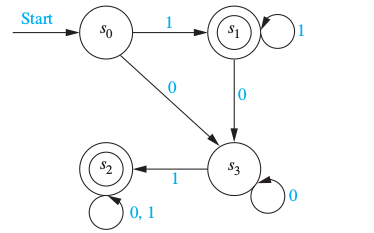
\includegraphics[width=\textwidth]{img/Q13_4_17}
\solution

$S \rightarrow 1A$\\ 
$S \rightarrow 0B$\\
$S \rightarrow 1$\\
$A \rightarrow 1A$\\
$A \rightarrow 0B$\\
$A \rightarrow 1$\\
$B \rightarrow 0B$\\
$B \rightarrow 1C$\\
$B \rightarrow 1$\\
$C \rightarrow 0C$\\
$C \rightarrow 1C$\\
$C \rightarrow 0$\\
$C \rightarrow 1$

\end{document}
